\documentclass[10pt, compress]{beamer}

\usetheme{m}

\usepackage{booktabs}
\usepackage[scale=2]{ccicons}
\usepackage{minted}

\usepackage[final]{pdfpages}
\usepackage{amsfonts}
\usepackage{tikz}

\usepackage{graphicx} 

% Define tikz styles here
\usetikzlibrary{fit, matrix, backgrounds, shapes, arrows}


\usepackage{listings}
\usepackage{caption}


\usemintedstyle{trac}

\title{A Hardware Implementation of a VQ Index Based Steganography Technique}
\subtitle{}
\date{\today}
\author{Inzamam Kaleem Rahaman}
\institute{University of the West Indies, St Augustine}

\begin{document}

\maketitle

\section{Background}

\begin{frame}[fragile]
  \frametitle{What is Steganography ?}

  %\begin{figure}
  %\centering
  %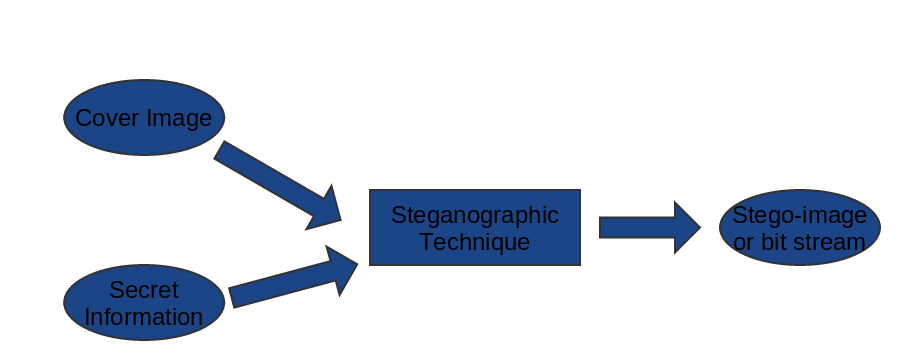
\includegraphics[scale=0.35]{steganography_summary.png}
  %%\label{fig:my_label}
  %\end{figure}
    
 % The \emph{mtheme} is a Beamer theme with minimal visual noise inspired by the
 % \href{https://github.com/hsrmbeamertheme/hsrmbeamertheme}{\textsc{hsrm} Beamer
 % Theme} by Benjamin Weiss.

  %Enable the theme by loading

%  \begin{minted}[fontsize=\small]{latex}
 %   \documentclass{beamer}
  %  \usetheme{m}
  %\end{minted}

  %Note, that you have to have Mozilla's \emph{Fira Sans} font and XeTeX
  %installed to enjoy this wonderful typography.
  
  \begin{figure}
        \scalebox{.8}{% Define block styles
\tikzstyle{decision} = [diamond, draw, fill=blue!20, 
    text width=6.7em, text badly centered, node distance=3cm, inner sep=0pt]
\tikzstyle{block} = [rectangle, draw, fill=blue!20, 
    text width=5em, text centered, rounded corners, minimum height=4em]
\tikzstyle{line} = [draw, -latex']
\tikzstyle{cloud} = [draw, ellipse,fill=red!20, node distance=3cm,
    minimum height=2em]
    
\begin{tikzpicture}[node distance = 4cm, auto]

    \node [block] (image-pre) {Cover Image};
   
     \node [decision, below of=image-pre,
     node distance=4cm] (feed) {Steganographic Technique};
      \node [block, below of=feed] (info) {secret information};
    \node [block, right of=feed] (end-res) {Stego-image or bitstream};
    
   
    % Place nodes
    %\node [block] (init) {initialize model};
    %\node [cloud, left of=init] (expert) {expert};
    %\node [cloud, right of=init] (system) {system};
    %\node [block, below of=init] (identify) {identify candidate models};
    %\node [block, below of=identify] (evaluate) {evaluate candidate models};
    %\node [block, left of=evaluate, node distance=3cm] (update) {update model};
    %\node [decision, below of=evaluate] (decide) {is best candidate better?};
    %\node [block, below of=decide, node distance=3cm] (stop) {stop};
    % Draw edges
    %\path [line] (init) -- (identify);
    %\path [line] (identify) -- (evaluate);
    %\path [line] (evaluate) -- (decide);
    %\path [line] (decide) -| node [near start] {yes} (update);
    %\path [line] (update) |- (identify);
    %\path [line] (decide) -- node {no}(stop);
    %\path [line,dashed] (expert) -- (init);
    %\path [line,dashed] (system) -- (init);
    %\path [line,dashed] (system) |- (evaluate);
    \path [line] (image-pre) -- (feed);
    \path[line] (info) -- (feed);
    \path[line] (feed) -- (end-res);
\end{tikzpicture}}
   \end{figure}
  
\end{frame}

\begin{frame}[fragile]
  \frametitle{What is an FPGA ?}
  
    \begin{figure}
        \scalebox{.8}{
\centering

\tikzstyle{switch}=[circle,
                                                thick,
                                                minimum size=0.9cm,
                                                draw=orange!80,
                                                fill=orange!25]

% The control input vector is represented by a purple circle.
\tikzstyle{input}=[rectangle,
                                    thick,
                                    minimum size=2.5cm,
                                    draw=purple!80,
                                    fill=purple!20]
                                    
\tikzstyle{background}=[rectangle,
                                                fill=gray!10,
                                                inner sep=0.2cm,
                                                rounded corners=5mm]

% The input, state transition, and measurement matrices
% are represented by gray squares.
% They have a smaller minimal size for aesthetic reasons.
\tikzstyle{matrx}=[rectangle,
                                    thick,
                                    minimum size=1cm,
                                    draw=gray!80,
                                    fill=gray!20]


\begin{tikzpicture}[>=latex,text height=1.5ex,text depth=0.25ex]
    % "text height" and "text depth" are required to vertically
    % align the labels with and without indices.
  
  % The various elements are conveniently placed using a matrix:
  \matrix[row sep=0.5cm,column sep=0.5cm] {
    % First line: Control input
    %&
        \node (lc1) [input]{logic cell}; &
        \node (s1)  [switch]{switch}; &
        \node (lc2) [input]{logic cell}; &
        \node (s2)  [switch]{switch}; &
        \node (lc3) [input]{logic cell}; &
        
        \\ 
        \node (s3) [switch]{switch}; &
        \node (s4) [switch]{switch}; &
        \node (s5)   [switch]{switch}; &
        \node (s6)   [switch]{switch}; &
        \node (s7) [switch]{switch}; &
        \\
         
        \node (lc4) [input]{logic cell}; &
        \node (s8)  [switch]{switch}; &
        \node (lc5) [input]{logic cell}; &
        \node (s9)  [switch]{switch}; &
        \node (lc6) [input]{logic cell}; &
        \\
    };
    
    % The diagram elements are now connected through arrows:
    \path[=]
        (lc1) edge[thick] (s1)
        (s1)  edge[thick] (lc2)
        (lc2) edge[thick] (s2)
        (s2) edge[thick] (lc3)
        (lc1) edge[thick] (s3)
        (s1) edge[thick] (s4)
        (lc2) edge[thick] (s5)
        (s2) edge[thick] (s6)
        (lc3) edge[thick] (s7)
        (s3) edge[thick] (s4)
        (s4) edge[thick] (s5)
        (s5) edge[thick] (s6)
        (s6) edge[thick] (s7)
        (s3) edge[thick] (lc4)
        (s4) edge[thick] (s8)
        (s5) edge[thick] (lc5)
        (s6) edge[thick] (s9)
        (s7) edge[thick] (lc6)
        (lc4) edge[thick] (s8)
        (s8) edge[thick] (lc5)
        (lc5) edge[thick] (s9)
        (s9) edge[thick] (lc6)
        ;
        
        
 \begin{pgfonlayer}{background}
        \node [background,
                    fit=(lc1) (lc6)] {};
    \end{pgfonlayer}
\end{tikzpicture}



%\caption{The general structure of an FPGA}
%\label{fig:fpga_structure}

}
        \caption{FPGA structure}
    \end{figure}
  %Sections group slides of the same topic

  %\begin{minted}[fontsize=\small]{latex}
   % \section{Elements}
  %\end{minted}

  %for which the \emph{mtheme} provides a nice progress indicator \ldots
\end{frame}

%\section{Elements}

\begin{frame}[fragile]
  \frametitle{What is an FPGA ?}
  
  \begin{figure}
  \centering
  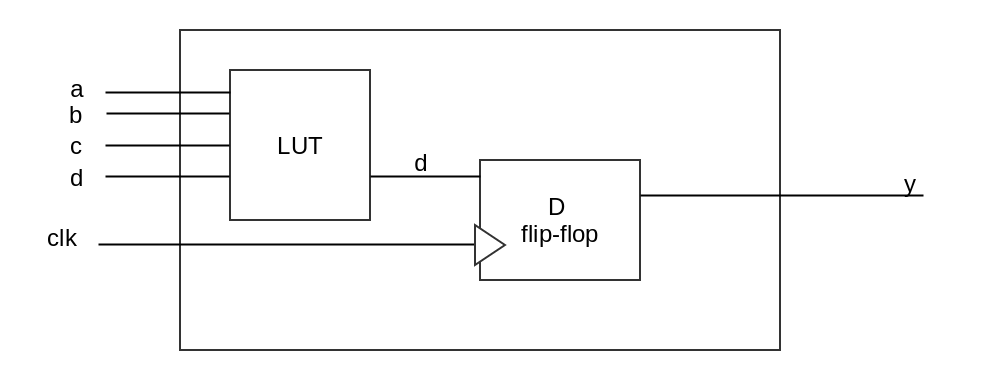
\includegraphics[scale=0.35]{logic_cell_structure.png}
  \caption{Internal structure of logic cell}
  %\label{fig:my_label}
  \end{figure}
  
\end{frame}


\section{Why Implement on an FPGA ?}

\begin{frame}{Why Implement on an FPGA ?}
    
    \begin{itemize}
        \item No Von Neumann Bottleneck
        \item No Context Switching
        \item Is more energy efficient than a software implementation
        \item Is a standalone component 
    \end{itemize}

\end{frame}

\section{Results}

\begin{frame}{Encoder State Machine}

    \begin{figure}
    \centering
    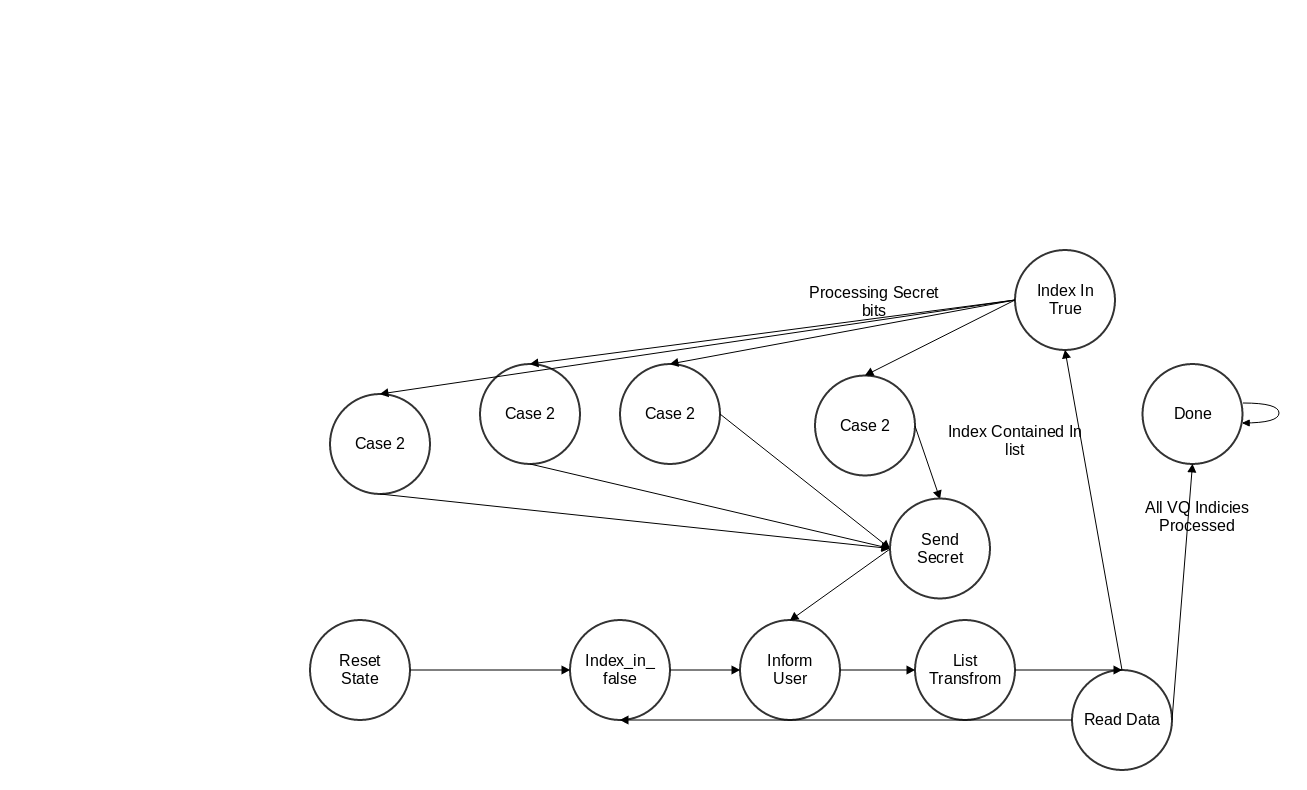
\includegraphics[scale=0.25]{encoder_states.png}
    \caption{State machine for encoder circuit}
    \end{figure}

\end{frame}

\begin{frame}{Encoder Circuit Overview}
    
    \begin{figure}
    \centering
    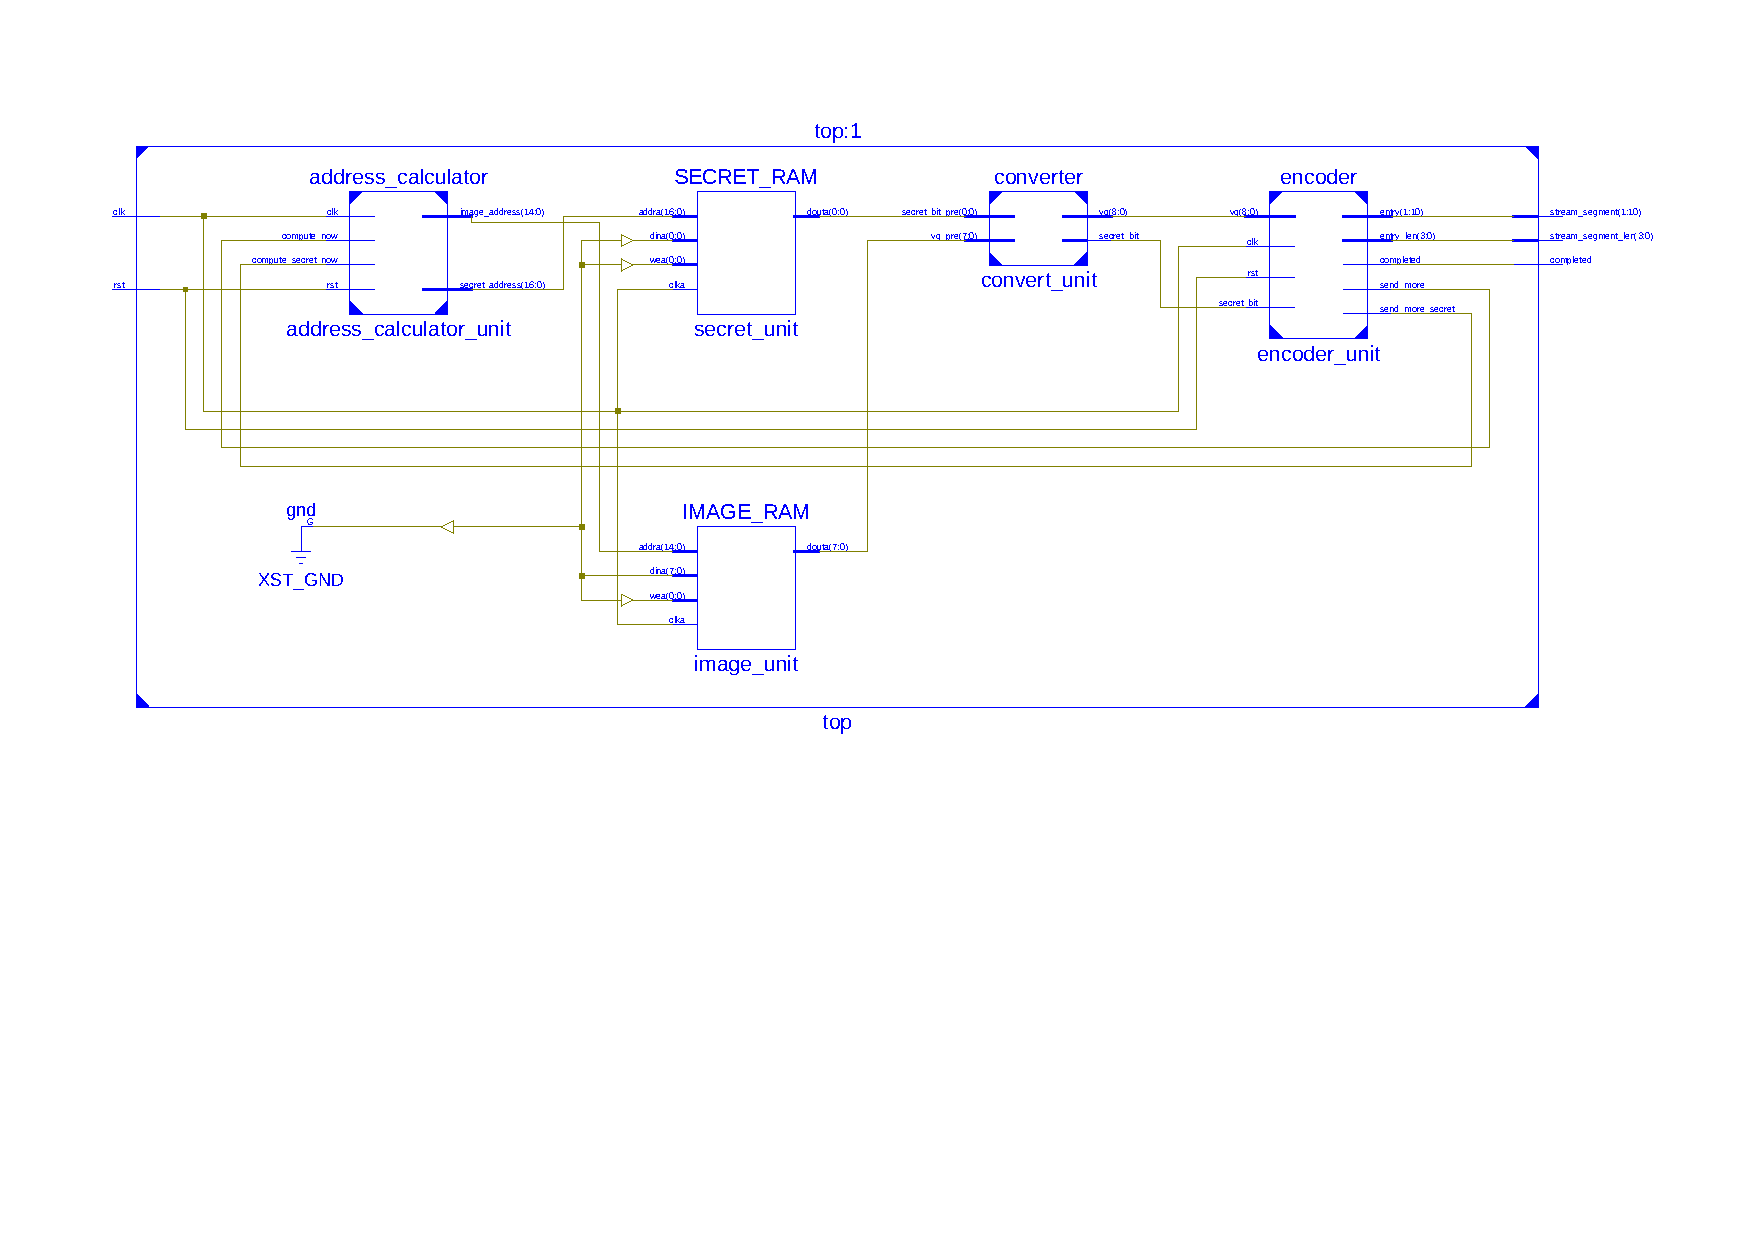
\includegraphics[scale=0.43]{top.pdf}
    \end{figure}
    

\end{frame}

\begin{frame}{Encoder Circuit Utilization}

    \begin{table}[h]
\begin{tabular}{llll}
\toprule
Logic Utilization          & Used & Available & Utilization \\ 
\midrule
Number of Slices           & 97   & 4656      & 2 \%        \\ 
Number of Slice Flip Flops & 125  & 9312      & 1 \%        \\ 
Number of 4 input LUTs     & 143  & 9312      & 1 \%        \\ 
Number of bonded IOBs      & 17   & 232       & 7 \%        \\ 
Number of BRAMs            & 15   & 20        & 75 \%       \\ 
Number of GCLKs            & 1    & 24        & 4 \%        \\ 
\bottomrule
\end{tabular}
\caption{Summary of resource utilization for encoder on XC3S500E}
%\caption{Summary of resource utilization}
%\label{table:util_summary}
\end{table}

\end{frame}


\begin{frame}{Encoder Timing Statistics}

\begin{table}[h]
\begin{tabular}{|l|l|}
\hline
Minimum period                           & 9.058 ns      \\ \hline
Maximum Frequency                        & 110.405 MHz   \\ \hline
Minimum input arrival time before clock  & 3.900 ns      \\ \hline
Maximum output required time after clock & 4.040 ns      \\ \hline
Maximum combinational path delay         & No Path found \\ 
\hline
\end{tabular}
\caption{Timing estimates for the encoder produced by the systhesis tool}
\end{table}
    

\end{frame}

\begin{frame}{Decoder State Machine}
    
    \begin{figure}
    \centering
    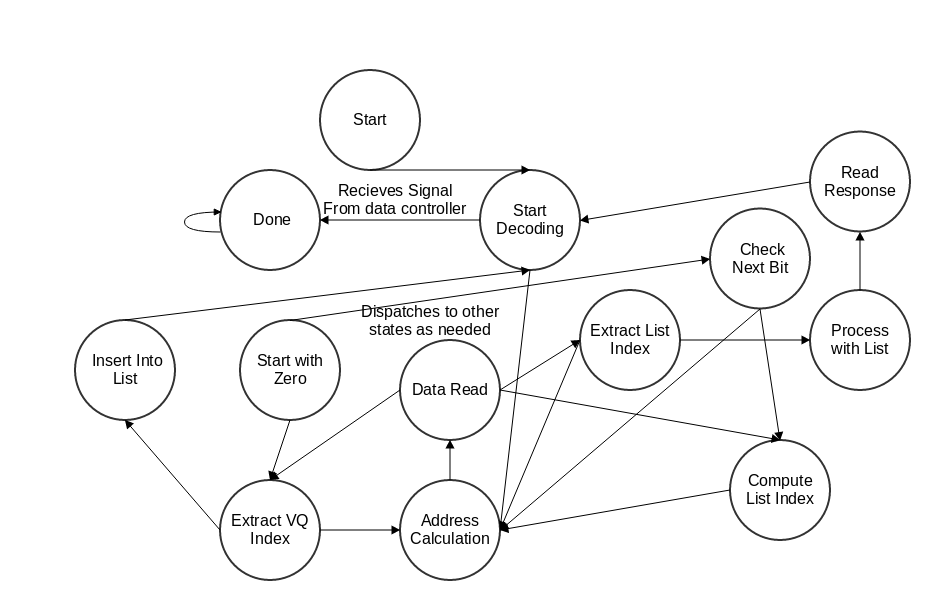
\includegraphics[scale=0.31]{decoder_states_v2.png}
    \caption{State machine for decoder circuit}
    \end{figure}
    

\end{frame}

\begin{frame}{Decoder Circuit Overview}

    \begin{figure}
    \centering
    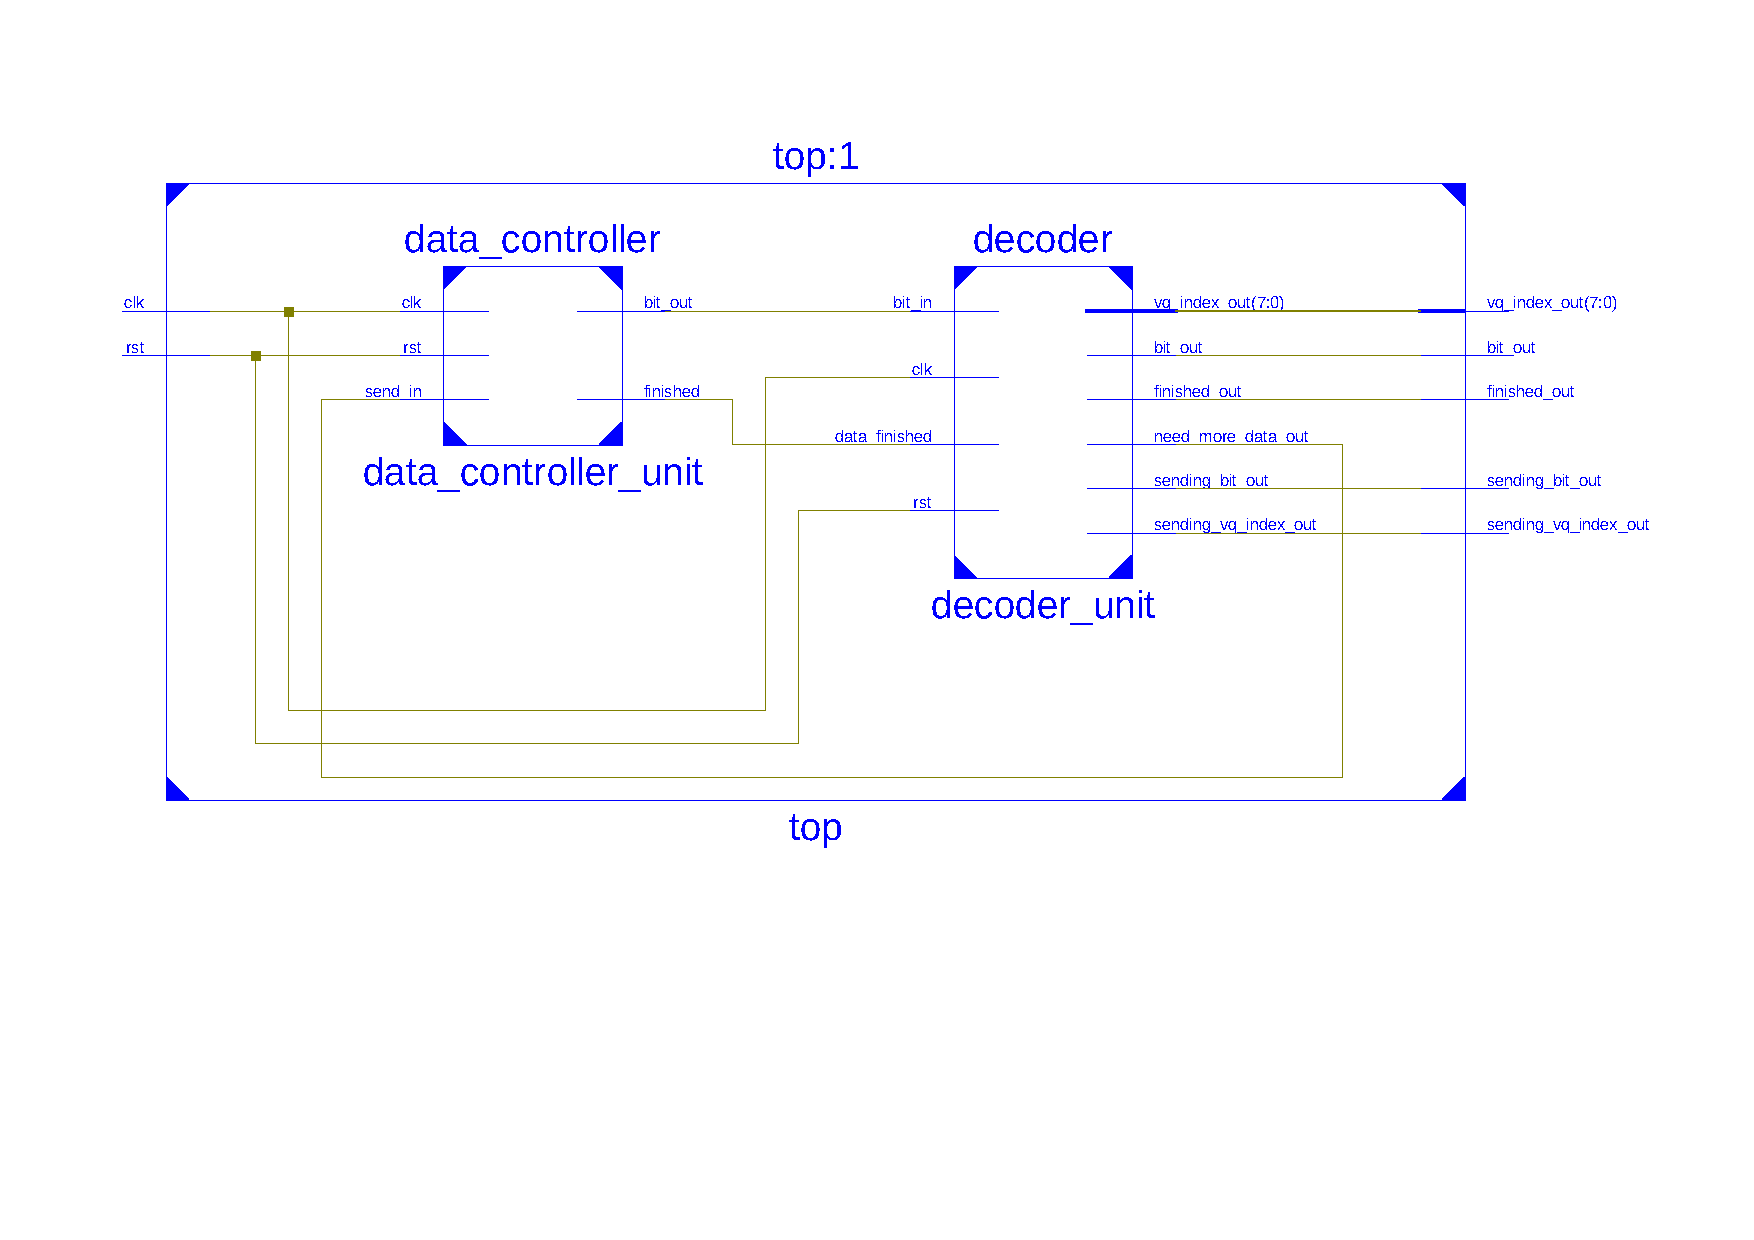
\includegraphics[scale=0.4]{decoder_top_diagram.pdf}
    \end{figure}    

\end{frame}


\begin{frame}{Decoder Circuit Utilization}

    \begin{table}[h]
\begin{tabular}{llll}
\toprule
Logic Utilization          & Used & Available & Utilization \\ 
\midrule
Number of Slices           & 152   & 4656      & 3 \%        \\ 
Number of Slice Flip Flops & 157  & 9312      & 1 \%        \\ 
Number of 4 input LUTs     & 285  & 9312      & 3 \%        \\ 
Number of bonded IOBs      & 14   & 232       & 6 \%        \\ 
Number of BRAMs            & 9   & 20        & 45 \%       \\ 
Number of GCLKs            & 1    & 24        & 4 \%        \\ 
\bottomrule
\end{tabular}
\caption{Summary of resource utilization for decoder on XC3S500E}
%\label{table:util_summary_decoder_2}
\end{table}

\end{frame}

\begin{frame}{Decoder Timing Statistics}

\begin{table}[h]
\begin{tabular}{|l|l|}
\hline
Minimum period                           & 8.067 ns      \\ \hline
Maximum Frequency                        & 123.967 MHz   \\ \hline
Minimum input arrival time before clock  & 4.371 ns      \\ \hline
Maximum output required time after clock & 4.040 ns      \\ \hline
Maximum combinational path delay         & No Path found \\ \hline
\end{tabular}
\caption{Timing estimates for the decoder produced by the systhesis tool}
\label{table:time_estimate_decoder}
\end{table}

\end{frame}



%\begin{frame}{Tables}
%  \begin{table}
%    \caption{Largest cities in the world (source: Wikipedia)}
%    \begin{tabular}{lr}
%      \toprule
%      City & Population\\
%      \midrule
%      Mexico City & 20,116,842\\
%      Shanghai & 19,210,000\\
%      Peking & 15,796,450\\
%      Istanbul & 14,160,467\\
%      \bottomrule
%    \end{tabular}
%  \end{table}
%\end{frame}
%\begin{frame}{Blocks}

 % \begin{block}{This is a block title}
  %  This is soothing.
  %\end{block}

%\end{frame}
%\begin{frame}{Math}
%  \begin{equation*}
%    e = \lim_{n\to \infty} \left(1 + \frac{1}{n}\right)^n
%  \end{equation*}
%\end{frame}
%\begin{frame}{Quotes}
%  \begin{quote}
%    Veni, Vidi, Vici
%  \end{quote}
%\end{frame}

%\plain{Dark background}{\vspace{-2em}\begin{center}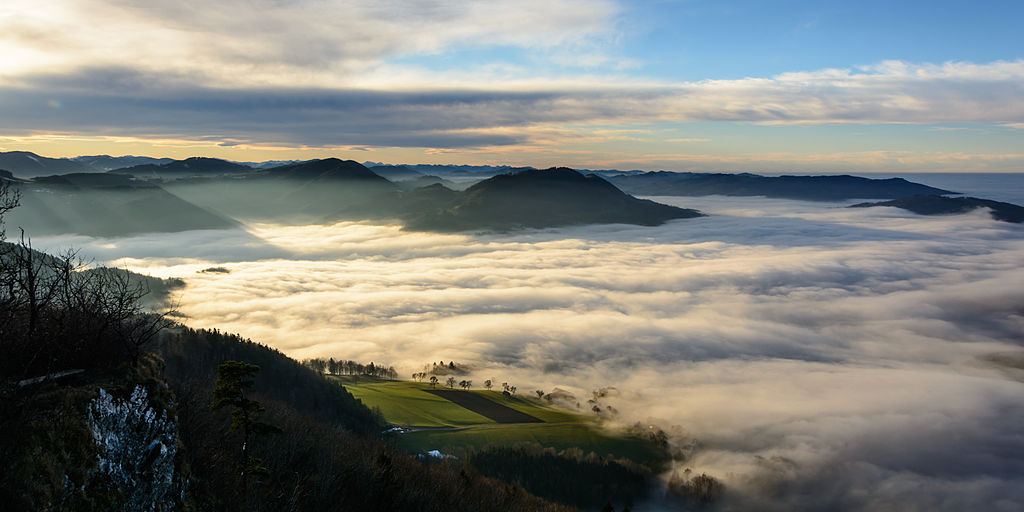
\includegraphics[width=\textwidth]{images/valley.jpg}\end{center}}




\plain{}{Questions?}

\end{document}
